\documentclass[useAMS,usenatbib,referee]{biom}

\usepackage{amsmath}
\usepackage[figuresright]{rotating}

\graphicspath{{include/}}

\def\bSig\mathbf{\Sigma}
\newcommand{\VS}{V\&S}
\newcommand{\tr}{\mbox{tr}}

\newcommand{\blind}{0} % 0 = not blind, 1 = blind

%\newcommand{\Stan}{{\tt Stan}}
\newcommand{\Stan}{Stan}
\newcommand{\RStan}{{\tt RStan}}
\newcommand{\edgeR}{{\tt edgeR}}
\newcommand{\baySeq}{{\tt baySeq}}
\newcommand{\ShrinkBayes}{{\tt ShrinkBayes}}
\newcommand{\RNAseq}{RNAseq}

\renewcommand{\gamma}{c}


\title{Empirical Bayes analysis of \RNAseq{} data for detection of gene expression heterosis}

\if0\blind{
\author{Jarad Niemi$^*$\email{niemi@iastate.edu}, 
Eric Mittman, 
Will Landau, and 
Dan Nettleton \\
Department of Statistics, Iowa State University, Ames, Iowa, U.S.A.}
} \fi

\begin{document}

\date{{\it Received December} 2014} 

\pagerange{\pageref{firstpage}--\pageref{lastpage}} 
\volume{VV}
\pubyear{YYYY}
\artmonth{MM}
\doi{x}

\label{firstpage}

\begin{abstract}
Heterosis, or hybrid vigor, refers to the enhancements in the phenotype of hybrid progeny relative to their inbred parents. Although the heterosis phenomenon is extensively utilized in agriculture, the molecular basis of heterosis is still largely unknown. In an effort to understand phenotypic heterosis at the molecular level, researchers have begun to measure transcript abundance levels of thousands of genes in parental inbred lines and their hybrid offspring using RNA sequencing (\RNAseq{}) technology.  The resulting data allow researchers to search for evidence of gene expression heterosis as one potential molecular mechanism underlying heterosis of agriculturally important traits.  The null hypotheses of greatest interest in testing for gene expression heterosis are composite null hypotheses that are difficult to test with standard statistical approaches for \RNAseq{} analysis. To address these shortcomings, we develop a hierarchical model based on a negativeb binomial data model and draw inferences using a computationally tractable empirical Bayes approach to inference. We demonstrate improvements over alternative methods via a simulation study based on a maize experiment and then analyze that maize experiment with our newly proposed methodology. This article has supplementary material online.
\end{abstract}

\begin{keywords}
Empirical Bayes; Gene expression; Heterosis; Hierarchical model; Negative binomial; \RNAseq{}.
\end{keywords}

\maketitle

%  A maximum of six (6) tables or figures combined is often required.''

\section{Introduction}
\label{s:intro}

Heterosis, or hybrid vigor, occurs when hybrid progeny display phenotypes that are superior to the phenotypes of their parents.  The heterosis phenomenon was scientifically documented in plants by \cite{darwin1876effects}and has long been used to improve agricultural production.  One classic example involves hybrid maize offspring that are taller, faster to mature, and yield considerably more grain than their inbred parents \citep{hallauer1981quantitative, hallauer2010quantitative}.  Despite intensive study and successful use of heterosis in agriculture, the basic molecular genetic mechanisms remain largely unknown \citep{coors1999genetics, lippman2007heterosis}. One potential explanation, known as gene expression heterosis, is enhanced expression of one or more genes in hybrids compared to their inbred parents \citep{swanson2006all, springer2007allelic}.

Recently, \cite{ji2014estimation} introduced an approach to assess gene expression heterosis using microarray data under the assumption that these data are continuous. They built a normal hierarchical model for microarray measurements of transcript abundance that allows borrowing of information across genes to estimate means and variances. They introduced an empirical Bayes framework that first estimates model hyperparameters, then estimates the posterior distribution for gene-specific parameters conditional on those hyperparameters, and finally computes heterosis probabilities based on integrals of regions under this posterior. This development was necessary due to the composite null hypotheses in tests for heterosis. These hypotheses, which many available methods do not fully accommodate, remain a challenge in the transition from continuous measurements of transcript abundance to count-based measurements that arise from RNA sequencing (\RNAseq{}) technology. Building on the work of \citeauthor{ji2014estimation} with the normal data model, we construct a hierarchical model based on a negative-binomial data model. We also utilize an empirical Bayes approach to obtain \emph{maximum a posterior} (MAP) estimates of the hyperparameters and the posterior distributions for the gene-specific parameters conditional on those hyperparameters. 

The remainder of the paper proceeds as follows. Section \ref{s:method} presents the proposed hierarchical model, an empirical Bayes method of estimating the parameters, and the calculation of posterior probabilities of gene expression heterosis. Section \ref{s:simulation} presents a simulation study based on a maize experiment and compares our approach to alternative methods. Section \ref{s:maize} analyzes a maize experiment where phenotypic heterosis is well established and identifies genes demonstrating expression heterosis. The data and code necessary to perform this analysis are available in the Supplemental Material. Section \ref{s:discussion} summarizes the work and suggests directions for future research.


\section{Empirical Bayes identification of gene expression heterosis from \RNAseq{} read counts}
\label{s:method}

An RNA sequencing (\RNAseq{}) experiment to identify genes demonstrating expression heterosis consists of three genetic varieties: two parental varieties (P1 and P2) and a cross between these two varieties called the hybrid (H). For each variety, replicate RNA samples are isolated and assessed for quality. Complementary DNA (cDNA) libraries, consisting of short cDNA fragments derived from RNA, are constructed. Then, next generation sequencing technology is used to determine the \emph{reads}, or nucleotide sequences, in the cDNA libraries. These reads are processed using bioinformatic algorithms to match the reads to genes, or specific gene transcripts, exons, microRNAs, etc. The results of read processing are summarized by a gene $\times$ sample matrix of counts. See \cite{datta2014statistical} for more details on \RNAseq{} experiments and data from a statistical perspective, and see \cite{paschold2012complementation} for the biological background behind the use of \RNAseq{} to study gene expression heterosis.

To use \RNAseq{} counts to identify genes displaying expression heterosis, we build a hierarchical model to borrow information across gene-variety means and across gene-specific overdispersion parameters, estimate the parameters using an empirical Bayes procedure implemented in the statistical software {\tt Stan}, and calculate empirical Bayes posterior probabilities for heterosis. 


\subsection{Hierarchical model for \RNAseq{} counts}
\label{s:model}

Let $Y_{gvi}$ be the count for gene $g=1,\ldots,G$, variety $v=1,\ldots,V$, and replicate $i=1,\ldots,n_v$.  We assume
\begin{equation} 
Y_{gvi} \stackrel{ind}{\sim} NB\left(e^{\mu_{gv}+\gamma_{vi}},e^{\psi_g}\right), 
\label{e:data}
\end{equation}
where $NB(\xi,e^\psi)$ indicates a negative binomial distribution with expectation $\xi$ and variance $\xi+e^\psi\xi^2$, and $ind$ indicates the observations are conditionally independent.  As shown in equation \eqref{e:data}, our data model involves gene-specific overdispersion $\psi_g$ and a mean that depends on the gene-variety combination through $\mu_{gv}$ and on the sample though  $\gamma_{vi}$.  The $\mu_{gv}$ terms are of primary scientific interest; the $\gamma_{vi}$ terms are normalization factors that account for differences in the thoroughness of sequencing from sample to sample. 

Following \cite{ji2014estimation}, we reparameterize the gene-variety mean structure into the gene-specific parental average ($\phi_g$), half-parental difference ($\alpha_g$), and hybrid difference ($\delta_g$). Specifically, for heterosis $V=3$ and let $v=1,2$ indicate the two parental varieties and $v=3$ indicate the hybrid, then
\[ \phi_g = \frac{\mu_{g1}+\mu_{g2}}{2}, \quad 
\alpha_g = \frac{\mu_{g1}-\mu_{g2}}{2}, \quad \mbox{and} \quad
\delta_g = \phi_g-\mu_{g3}. \]

We present a hierarchical model for the gene-specific mean parameters and overdispersion parameters. The parental averages and overdispersion parameters are assumed to follow a normal distribution, i.e.
\[ 
%\gamma_{vi} \stackrel{ind}{\sim} N(0,\sigma_\gamma^2), \quad 
\phi_g \stackrel{ind}{\sim} N(\eta_\phi, \sigma_\phi^2), \quad \mbox{and}\quad 
\psi_g \stackrel{ind}{\sim} N(0,\sigma_\psi^2). 
\]
To allow for more shrinkage with the half-parental and hybrid differences, we use a Laplace (or double exponential prior) and thus implement a Bayesian LASSO \citep{park2008bayesian}, i.e. 
\[ 
\alpha_g \stackrel{ind}{\sim} La(\eta_\alpha, \sigma_\alpha) \qquad \mbox{and} \qquad
\delta_g \stackrel{ind}{\sim} La(\eta_\delta, \sigma_\delta) 
\]
where $\alpha\sim La(\eta,\sigma)$ has a probability density function given by $p(\alpha|\eta,\sigma) = \exp(-|\alpha-\eta|/\sigma)/2\sigma$ with expectation $\eta$ and variance $2\sigma^2$. We assume independence amongst the normalization factors, parental averages, half parental differences, hybrid differences, and overdispersion parameters.

We assume improper uniform priors for $\eta_\phi$, $\eta_\alpha$, and $\eta_\delta$ and independent half-cauchy priors for all standard deviations \citep{gelman2006prior}.

\subsection{Empirical Bayes}
\label{s:ebayes}

We separate the parameters of the model in Section \ref{s:model} into gene-specific parameters $\theta = (\theta_1,\ldots,\theta_G)$ where $\theta_g = (\phi_g,\alpha_g,\delta_g,\psi_g)$ and hyperparameters $\pi = (\gamma, \eta, \sigma)$, where $\gamma = (\gamma_{11},\ldots,\gamma_{Vn_V})$, $\eta=(\eta_\phi,\eta_\alpha,\eta_\delta)$, and $\sigma=(\sigma_\gamma,\sigma_\phi,\sigma_\alpha,\sigma_\delta,\sigma_\psi)$. We employ an optimization procedure to obtain the \emph{maximum a posteriori} (MAP) estimate for $\pi$, denoted $\hat{\pi}$, and then base gene-specific inference on the posterior conditional on this MAP estimate. Conditional on the hyperparameters, the gene-specific parameters are independent, i.e., 
\begin{equation}
\begin{split}
p\left(\theta\left|y,\hat{\pi}\right.\right) 
%&= \prod_{g=1}^G p\left(\theta_g\left|y_g,\hat{\pi}\right.\right) = \prod_{g=1}^G p\left(y_g\left|\theta_g,\hat{\gamma}\right.\right) p\left(\theta_g\left|\hat{\pi}\right.\right) \nonumber \\
%&\propto \prod_{g=1}^G \left[ \prod_{v=1}^V \prod_{i=1}^{n_v} NB\left(y_{gvi}\left|e^{\mu_{gv}+\hat{\gamma}_{vi}},e^{\psi_g}\right.\right) \right] p(\theta_g|\hat{\eta},\hat{\sigma}) \\
\propto \prod_{g=1}^G & \left[ \,\prod_{v=1}^V \prod_{i=1}^{n_v} NB\left(y_{gvi};e^{\mu_{gv}+\hat{\gamma}_{vi}},e^{\psi_g}\right)  \right. \\
&\times 
\left. \vphantom{\prod_{v=1}^V}
N(\phi_g;\hat{\eta}_\phi, \hat{\sigma}_\phi^2)
La(\alpha_g;\hat{\eta}_\alpha, \hat{\sigma}_\alpha)
La(\delta_g;\hat{\eta}_\delta, \hat{\sigma}_\delta)
N(\psi_g;\hat{\eta}_\psi, \hat{\sigma}_\psi^2) 
\right]
\label{e:condind}
\end{split}
\end{equation}
Thus, conditional posterior inference for the gene-specific parameters can be obtained independently and in parallel.

As we have not integrated out the gene-specific parameters when obtaining the MAP estimate, we actually receive a joint MAP estimate of $\theta$ and $\pi$. We explicitly use the MAP estimate of $\pi$ when obtaining empirical Bayes posterior samples for the gene-specific parameters as in equation \eqref{e:condind}. The MAP estimate of $\theta$ could be used as initial values in the MCMC, although we did not find this necessary.

\subsection{Gene expression heterosis}
\label{s:gene_heterosis}

For a specific gene $g$, low-parent heteorisis (LPH) of gene expression occurs when average expression in the hybrid is less than the average expression of either parent, i.e. $\delta_g < -|\alpha_g|$, and high-parent heterosis (HPH) occurs when average expression in the hybrid is greater than the average expression of either parent, i.e. $\delta_g > |\alpha_g|$. 
% and high-parent  heterosis (HPH) of gene expression occurs when $\max(\mu_{g1},\mu_{g2}) < \mu_{g3}$. For simplicity, we define \emph{heterosis} of gene expression to be the event of LPH or HPH. The most important hypotheses are
% \begin{align}
% H_{g0}:&\mu_{g1}\le \mu_{g3}\le \mu_{g2} \mbox{ or } \mu_{g1}\ge \mu_{g3}\ge \mu_{g2} \mbox{\ \ vs.\ \ } \nonumber \\
% H_{g1}:&\mu_{g3}< \min(\mu_{g1},\mu_{g2}) \mbox{ or } \max(\mu_{g1},\mu_{g2}) < \mu_{g3},
% \label{e:hypotheses}
% \end{align}
% where $H_{g0}$ indicates no heterosis for gene $g$ and $H_{g1}$ indicates  heterosis for gene $g$. 
% We evaluate these hypotheses based on empirical Bayes estimates of their posterior probabilities, e.g., 
% \begin{align}
% P\left(H_{g1}|y, \hat{\pi}_{MAP}\right) &= P\left(\left.\mu_{g3}< \min(\mu_{g1},\mu_{g2}) \mbox{ or } \max(\mu_{g1},\mu_{g2}) < \mu_{g3}\right| y, \hat{\pi}_{MAP}\right) \nonumber \\
% &\approx \frac{1}{M} \sum_{m=1}^M \mathrm{I}\left(\mu_{g3}^{(m)}< \min\left(\mu_{g1}^{(m)},\mu_{g2}^{(m)}\right) \mbox{ or } \max\left(\mu_{g1}^{(m)},\mu_{g2}^{(m)}\right) < \mu_{g3}^{(m)}\right), \label{e:probs}
% \end{align}
% where $\mu_g^{(m)} = \left(\mu_{g1}^{(m)},\mu_{g2}^{(m)},\mu_{g3}^{(m)}\right)$ is the $m^{th}$ MCMC sample from the empirical Bayes posterior, and $\mathrm{I}(A)$ is 1 if A is true and 0 otherwise. 
We evaluate these probabilities based on empirical Bayes estimates of their posterior probabilities, e.g., 
\begin{equation}
%P(LPH_g|y) \approx 
P(LPH_g|y,\hat{\pi}_{MAP}) = P\left(\left.\delta_g < -|\alpha_g|\right|y, \hat{\pi}_{MAP}\right) = \frac{1}{M} \sum_{m=1}^M \mathrm{I}\left(\delta_g^{(m)} < -\left|\alpha_g^{(m)}\right|\right), 
\label{e:probs}
\end{equation}
where $\left(\delta_g^{(m)},\alpha_g^{(m)}\right)$ is the $m^{th}$ MCMC sample from the empirical Bayes posterior, and $\mathrm{I}(A)$ is 1 if A is true and 0 otherwise. HPH probability is defined similarly with the inequality reversed and without the negative sign. We construct a ranked list of genes according to the maximum of the gene's LPH and HPH heterosis probabilities. Geneticists can use this list to prioritize future experiments to understand the molecular genetic mechanisms for heterosis.  
 

\subsection{Implementation in \Stan{}}

To perform the optimization required for the MAP estimate $\hat{\pi}$, we use the statistical software, {\tt Stan} \citep{stan-software:2014}, executed through the \RStan{} interface \citep{rstan-software:2014} in R \citep{R2014}. The Stan software allows the construction of general Bayesian models with the primary restriction that all unknown parameters are continuous. With a fully constructed model, the software can obtain MAP estimates \cite[Section 50.3,][]{stan-manual:2014} using the {\tt optimizing} function in \RStan{}. Presumably due to the large dimension of the optimization, it was necessary to use the L-BFGS algorithm \cite[Section 55,][]{stan-manual:2014} and reasonable starting values obtained via \edgeR{} \citep{robinson2010edgeR} from Bioconductor \citep{gentleman2004bioconductor}. The {\tt Stan} software also includes the \RStan{} function, {\tt sampling}, an implementation of a Markov chain Monte Carlo (MCMC) algorithm for obtaining samples from the posterior. By default, Stan uses a no-U-turn sampler \citep{hoffman2013no}, a variant of Hamiltonion Monte Carlo \citep{neal2011mcmc}.


\subsection{Implementation in \ShrinkBayes{}}

\ShrinkBayes{} utilizes integrated nested Laplace approximation (INLA) \citep{rue2009approximate} in combination with empirical Bayes ideas \citep{van2014shrinkbayes}. One limitation with inferential methods based on INLA is that all distributions, except for the data distribution, must have tails as light or lighter than the normal density. Thus, we cannot implement the Laplace priors for the half-parental difference ($\alpha_g$) and the hybrid difference ($\delta_g$) and instead use normal priors in this situation. An additional limitation is that INLA provides approximations to marginal posteriors for parameters or linear combinations of parameters, but not an approximation to the full posterior. Since we are interested in non-linear quantities such as $P(\delta_g > |\alpha_g||y)$, we cannot compute these directly using \ShrinkBayes{}. Instead, for \ShrinkBayes{}, we calculate heterosis probabilities conditional on posterior means for $\hat{\delta}_g$ and $\hat{\alpha}_g$, e.g. 
\[ 
% P_{\ShrinkBayes{}}(LPH_g|y) \equiv \left\{ \begin{array}{ll}
% P(\delta_g>-\alpha_g|y) & \mbox{if } \hat{\delta}_g > -\hat{\alpha}_g \ge 0 \\
% P(\delta_g>\phantom{-}\alpha_g|y) & \mbox{if } \hat{\delta}_g > \phantom{-}\hat{\alpha}_g \ge 0 \\
% 0 & \mbox{otherwise}
% \end{array} \right.
P_{\ShrinkBayes{}}(LPH_g|y) \equiv P(\delta_g>-\alpha_g|y)\mathrm{I}\left(\hat{\delta}_g > -\hat{\alpha}_g \ge 0\right) + P(\delta_g>\alpha_g|y) \mathrm{I}\left(\hat{\delta}_g > \hat{\alpha}_g \ge 0\right).
%P_{\ShrinkBayes{}}(HPH|y) \equiv \left\{ \begin{array}{ll}
%P(\delta_g<-\alpha_g|y) & \mbox{if } \hat{\delta}_g > -\hat{\alpha}_g \ge 0 \\
%(\delta_g<\phantom{-}\alpha_g|y) & \mbox{if } \hat{\delta}_g > \phantom{-}\hat{\alpha}_g \ge 0 \\
%0 & \mbox{otherwise}
%\end{array} \right.
\]
HPH probability is defined similarly with all inequalities reversed. As before, we construct a ranked list of genes according to the maximum of the gene's LPH and HPH heterosis probabilities.
%the heterosis probability for gene $g$ is zero if $|\hat{\delta}_g| \le |\hat{\alpha}_g|$, $P(\delta_g>\alpha_g|y)$ if $\hat{\delta}_g > -\hat{\alpha}_g \ge 0$, $P(\delta_g - \alpha_g > 0 |y)$ if $\hat{\delta}_g > \hat{\alpha}_g \ge 0$, $P(\delta_g - \alpha_g < 0 |y)$ if $\hat{\delta}_g < \hat{\alpha}_g \le 0$, and $P(\delta_g + \alpha_g < 0 |y)$ if $\hat{\delta}_g < -\hat{\alpha}_g \le 0$.  



\section{Simulation study based on a maize experiment}
\label{s:simulation}

% \subsection{Coverage for our model}
% \input{../temp/analyze-heterosis/FIGURES/coverage}

To assess the efficacy of our method to identify genes demonstrating heterosis, we used a maize data set with parental varieties B73 and Mo17 and the hybrid variety (B73 $\times$ Mo17) \citep{paschold2012complementation} to determine realistic parameter values for a simulation study. Section \ref{s:maize} describes the maize dataset in detail. We compared our method to approaches using the R packages \edgeR{}, \baySeq{} \citep{hardcastle2010bayseq, hardcastle2012baySeq}, and \ShrinkBayes{} \citep{van2014shrinkbayes}.

\subsection{Constructing simulated data}
\label{s:sim_data}

We applied the \edgeR{} package \citep{robinson2010edgeR} from Bioconductor \citep{gentleman2004bioconductor} to the maize data on 27,888 genes with average count at least one and at most two zero read counts for each variety across four replications.  This analysis produced sample-specific normalization factors using the TMM method \citep{robinson2010scaling},
%(0.080, -0.041, -0.054, 0.000, -0.036, -0.147, 0.093, 0.059, -0.004, -0.057, 0.067,  0.041) 
gene-specific dispersion estimates, and gene-variety-specific location parameter estimates \citep{mccarthy2012differential}. We treated these estimates as the true parameter values for the simulation study so that our simulated datasets mimicked the existing covariance structure among the gene-variety means of the original maize data.

Using these parameters and normalization factors, we simulated data according to the negative-binomial model in \eqref{e:data} independently for each gene. For each simulation, we analyzed a subset of 25,000 genes selected randomly from genes with simulated counts at least one on average and with at most two zeros for each variety across replications.  We repeated this simulation process 10 times for each of 4, 8, and 16 replicates per variety, reusing normalization factors when necessary.  
% From Dan "Did we consider changing the number of zeros allowed when the number of reps is higher?  I like the idea of simplifying all this by just picking an average count threshold that his high enough to avoid problems.  I think that may be what others have done in the past."

\subsection{Alternative methods}
\label{s:alternative}

Existing \RNAseq{} data analysis methods are not specifically designed to identify gene expression heterosis, but we adapted the approaches in \edgeR{} and {\tt baySeq} to provide a measure of the strength of heterosis for each gene such that large values of this measure indicate support for heterosis.

\edgeR{} can be used to test for differential expression between any two varieties based on the fit of a negative binomial log-linear model \citep{robinson2007moderated, robinson2010edgeR}. To construct a measure of heterosis, we computed the maximum likelihood estimates of the $\mu_{gv}$ parameters for all genes using \edgeR{}'s built-in Fisher scoring algorithm, and then used likelihood ratio tests to calculate two $p$-values for each gene: $p_{g1}$  for testing $H_{g01}:\mu_{g1}=\mu_{g3}$ and $p_{g2}$ for testing $H_{g02}:\mu_{g2}=\mu_{g3}$. Then, for each gene, we define a new $p$-value denoted as $p_g$ and determined as $p_g=1$ if the estimate of $\mu_{g3}$ falls between the estimates of $\mu_{g1}$ and $\mu_{g2}$ and $p_g=\max\{p_{g1},p_{g2}\}/2$ otherwise.  (For all relevant signifcance thresholds $\omega$ near 0, it can be shown that rejecting the null hypothesis of no heterosis of expression for gene $g$ whenever $p_g\leq \omega$ results in a test that is asymptotically size $\omega$.)  We then use $1-p_g$ as a final measure positively associated with strength of evidence for gene expression heterosis. 

{\tt baySeq} allows for a wider range of hypotheses for each gene, including $H^*_{g1}: \mu_{g1}=\mu_{g2}=\mu_{g3}$, $H^*_{g 2}: \mu_{g1}=\mu_{g2}$, $H^*_{g 3}: \mu_{g1}=\mu_{g3}$, $H^*_{g 4}: \mu_{g2}=\mu_{g3}$, and $H^*_{g 5}:$ all $\mu_g$'s are distinct. In a technique similar to our application of \edgeR{}, we used the posterior probabilities of these hypotheses to construct a measure of heterosis for each gene. We set this measure to zero if the maximum likelihood estimate, calculated using \edgeR{}, of $\mu_{g3}$ is between the maximum likelihood estimates of $\mu_{g1}$ and $\mu_{g2}$. Otherwise, the measure is the sum of the posterior probabilities of $H^*_{g 2}$ and $H^*_{g 5}$, the only hypotheses that allow for heterosis.



\subsection{Results}

For each of the methods above, as well as the method described in Section \ref{s:gene_heterosis}, we sorted genes according to the computed measure of the strength of evidence for heterosis. From these sorted lists, we constructed receiver-operating characteristic (ROC) curves to evaluate the ability of these methods to distinguish genes with heterosis, as defined in Section \ref{s:sim_data}, 
% From Dan, "why this citation?"
from those without heterosis \citep{landau2013dispersion}. A representative set of ROC curves is shown in Figure \ref{f:roc}. 
\begin{figure}[htbp]
\centerline{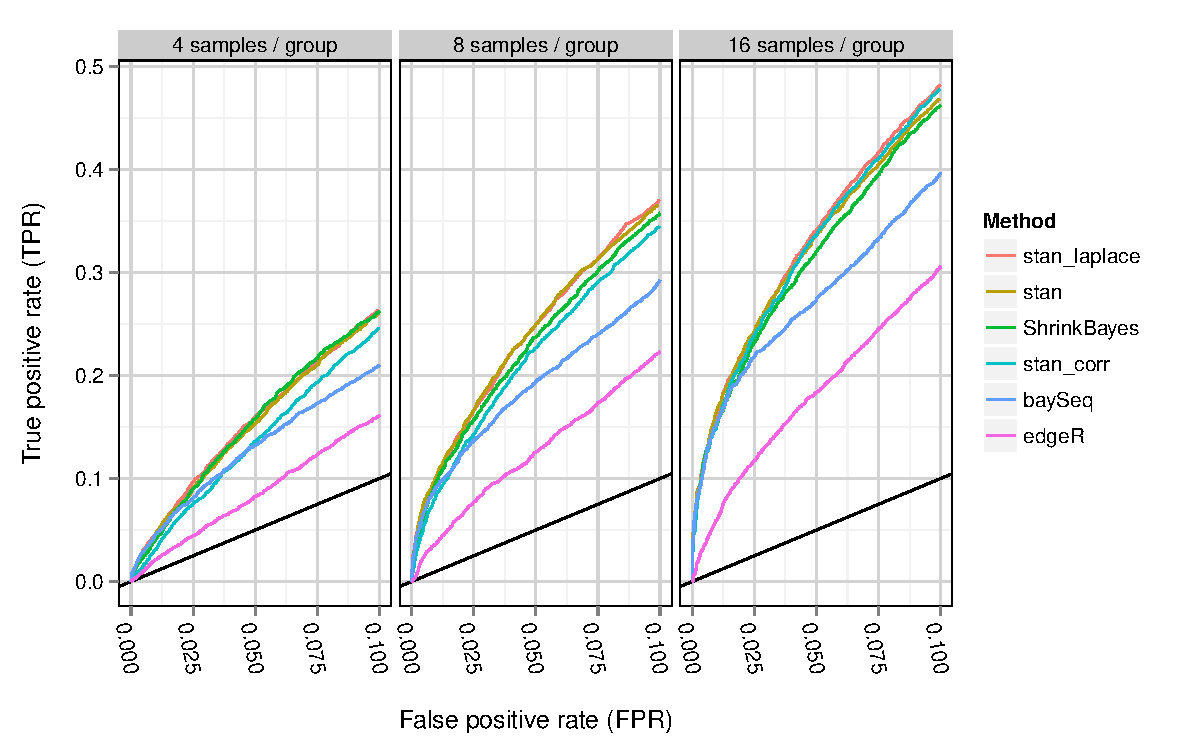
\includegraphics[width=\textwidth]{exampleROC0_1}}
\caption{Representative ROC curves for false positive rates below 0.1 for the approaches using \edgeR{}, {\tt baySeq},  and \ShrinkBayes{} described in Section \ref{s:alternative}, along with the independence and dependence methods using \RStan{} described in Section \ref{s:gene_heterosis}.}
\label{f:roc}
\end{figure}
For this simulation, we can see that the approaches based on the model in Section \ref{s:model}, i.e. \RStan{} and \ShrinkBayes{}, provide the best true positive rate for a given false positive rate. Also, as expected, as the sample size increases, our ability to distinguish genes with heterosis from genes without improves.


Figure \ref{f:auc} provides the area under the ROC curve below a false positive rate of 0.1 across the 10 simulations for each of the 3 different sample sizes. 
\begin{figure}
\centerline{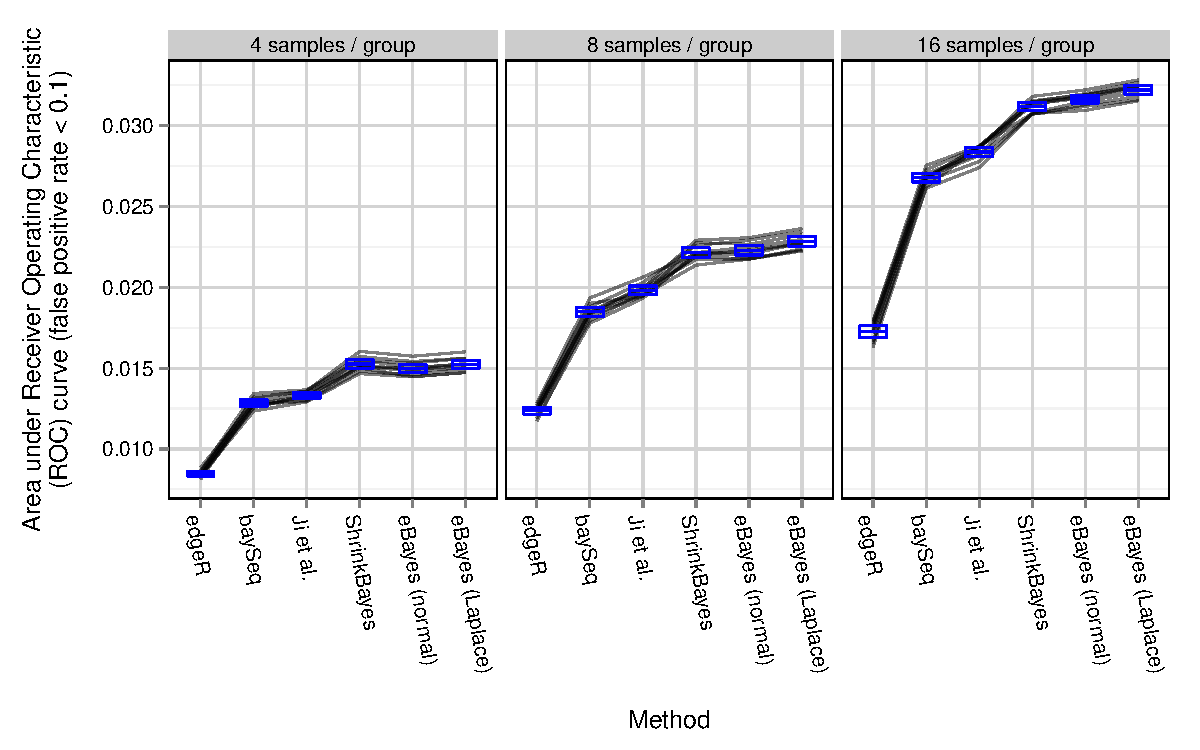
\includegraphics[width=\textwidth]{auc-facet-TRUE}}
\caption{Area under the ROC curves below a false positive rate of 0.1 for 3 different sample sizes for the approaches using \edgeR{}, {\tt baySeq},  and \ShrinkBayes{} described in Section \ref{s:alternative} , along with the independence and dependence methods using \RStan{} described in Section \ref{s:gene_heterosis}. Each line is a different simulation while the blue box indicates mean AUC and mean AUC plus and minus one standard error across the simulations.}
\label{f:auc}
\end{figure}
The pattern appears to hold, with the \RStan{} and \ShrinkBayes{} techniques outperforming the other two. %While there does not appear to be a significant difference between \ShrinkBayes{} and the independence model using \RStan{}, performance for \RStan{} appears to decrease for the dependence model where an unstructured covariance is estimated, at least for smaller sample sizes.



\section{Searching for gene expression heterosis in the maize experiment}
\label{s:maize}

We used our method to analyze the maize data set, generated by \cite{paschold2012complementation}, on gene expression in parental lines B73 and Mo17 and the hybrid genotype (B73$\times$Mo17). The data are available in the Supplemental Materials. Each variety had four biological replicates measured with Illumina methodology and equipment. Reads were mapped to the whole reference genome using the short reads aligner, NOVOALIGN. For more specifics, please see \cite{paschold2012complementation}. 

As explained in Section~\ref{s:sim_data}, we analyzed a set of $G=27,888$ genes for $V=3$ varieties and $n_v=4$ replicates ($v=1,2,3$). 

We found MAP estimates for both the independence and dependence models as shown in Table \ref{t:map}. 
% latex table generated in R 3.1.2 by xtable 1.7-4 package
% Fri Dec 19 08:07:56 2014
\begin{table}[ht]
\centering
\caption{MAP estimates for hyperparameters in the independent model and model with an estimated covariance based on the maize experiment data.} 
\label{t:map}
\begin{tabular}{l|rr|}
  \hline
 & Independent & Covariance \\ 
  \hline
$\eta_1$ & 4.62 & 4.61 \\ 
  $\eta_2$ & 4.68 & 4.66 \\ 
  $\eta_3$ & 4.72 & 4.70 \\ 
  $\eta_4$ & -3.14 & -2.40 \\ 
   \hline
$\sigma_1$ & 1.90 & 2.00 \\ 
  $\sigma_2$ & 1.80 & 1.90 \\ 
  $\sigma_3$ & 1.77 & 1.86 \\ 
  $\sigma_4$ & 0.78 & 0.59 \\ 
   \hline
$\rho_{12}$ &  & 0.90 \\ 
  $\rho_{13}$ &  & 0.97 \\ 
  $\rho_{14}$ &  & -0.35 \\ 
  $\rho_{23}$ &  & 0.96 \\ 
  $\rho_{24}$ &  & -0.31 \\ 
  $\rho_{34}$ &  & -0.34 \\ 
   \hline
$\tau$ & 0.06 & 0.07 \\ 
   \hline
$\gamma_{1}$ & 0.09 & 0.07 \\ 
  $\gamma_{2}$ & -0.02 & -0.04 \\ 
  $\gamma_{3}$ & -0.03 & -0.06 \\ 
  $\gamma_{4}$ & 0.03 & 0.00 \\ 
  $\gamma_{5}$ & -0.02 & -0.04 \\ 
  $\gamma_{6}$ & -0.12 & -0.14 \\ 
  $\gamma_{7}$ & 0.11 & 0.08 \\ 
  $\gamma_{8}$ & 0.08 & 0.06 \\ 
  $\gamma_{9}$ & 0.01 & -0.01 \\ 
  $\gamma_{10}$ & -0.03 & -0.05 \\ 
  $\gamma_{11}$ & 0.09 & 0.06 \\ 
  $\gamma_{12}$ & 0.07 & 0.04 \\ 
   \hline
\end{tabular}
\end{table}

The MAP estimates for the hierarchical means, $\eta$, and standard deviations, $\sigma$, are consistent between the independence and dependence models with, perhaps, a slightly larger mean and smaller standard deviation for the logarithm of the overdispersion parameter, $\psi_g$, in the dependence model relative to the independence model. In the dependence model, there appears to be high correlation amongst $\mu_{g1}$, $\mu_{g2}$, and $\mu_{g3}$, and negative correlation between $\psi_g$ and each of $\mu_{g1}$, $\mu_{g2}$, and $\mu_{g3}$. The normalization factors, and their variance, are consistent between the two models, with the estimates for the dependence model being consistently 0.02 larger than the estimates for the independence model, and both indicating that there is about a 25\% increase in counts between the least and most thoroughly sequenced samples. 


Independently for each gene, we ran four Markov chains conditional on the estimated hyperparameters to obtain approximate posterior distributions for all gene-specific parameters. Each Markov chain used initial values randomly drawn by {\tt Stan} and was run for a total of 2000 iterations, with 1000 iterations of burn-in and the remaining 1000 draws thinned by a factor of 4 for storage reasons. 
% From Dan "Do we need to be more specific about what method was used to generate the chains?"
The potential scale reduction factor, $\hat{R}$, was computed for each parameter \citep{Gelm:Rubi:infe:1992, Broo:Gelm:gene:1997}. If the maximum $\hat{R}$ was larger than 1.1 for any parameter, the total number of iterations was increased by 500, with the burn-in increased proportionally, and the chain was rerun. This process was repeated until the maximum $\hat{R}$ was less than 1.1 for all parameters.

With posteriors for all parameters, we can calculate empirical Bayes posterior probabilities for LPH and HPH. For each gene, the quantity of interest is likely to be the maximum of these two probabilities. For each gene with a high probability of either HPH or LPH, the magnitude of the effect is of interest. We calculate 
\begin{equation}
% \mbox{estimated effect size}_g = \left\{ 
% \begin{array}{ll}
% \hat{\mu}_{g3} - \min(\hat{\mu}_{g1},\hat{\mu}_{g2}) & \mbox{if } \hat{\mu}_{g3} < \min(\hat{\mu}_{g1},\hat{\mu}_{g2}) \\
% \hat{\mu}_{g3} - \max(\hat{\mu}_{g1},\hat{\mu}_{g2}) & \mbox{if } \hat{\mu}_{g3} > \max(\hat{\mu}_{g1},\hat{\mu}_{g2}) \\
% 0 & \mbox{otherwise},
% \end{array} 
% \right. 
\mbox{estimated effect size}_g \equiv \left\{ 
\begin{array}{ll}
\hat{\delta}_g - |\hat{\alpha}_g| & \mbox{if } \hat{\delta}_g > \phantom{-}|\alpha_g| \\
\hat{\delta}_g + |\hat{\alpha}_g| & \mbox{if } \hat{\delta}_g < -|\alpha_g| \\
0 & \mbox{otherwise},
\end{array} 
\right. 
\label{e:effect_size}
\end{equation}
where $\hat{\mu}_{gi}$ is the estimated posterior mean of $\mu_{gv}$ for $v=1,2,3$. Thus, the estimated effect size is the difference between hybrid mean and the nearest parent with negative values indicating LPH and positive values indicating HPH. If the hybrid mean is estimated to be between the parents, this effect is defined to be zero. 


Figure \ref{f:volcano} provides a volcano plot, in this case a bivariate histogram, to visualize the maximum of the probabilities of LPH and HPH versus estimated effect size. The figure shows a peak at zero for probabilities below 0.5 with estimated effect sizes of zero. Above a probability of 0.5, we see a prototypical volcano pattern, with increased heterosis probability corresponding to larger estimated effect sizes and no estimated effect sizes near zero for genes with high heterosis probability. We also see asymmetry, with larger negative effect sizes than positive effect sizes due to genes with hybrid counts near zero and relatively high parental counts. Genes with high estimated posterior probabilities of heterosis and large estimated effect sizes are candidates for further investigation.

\begin{figure}
\centerline{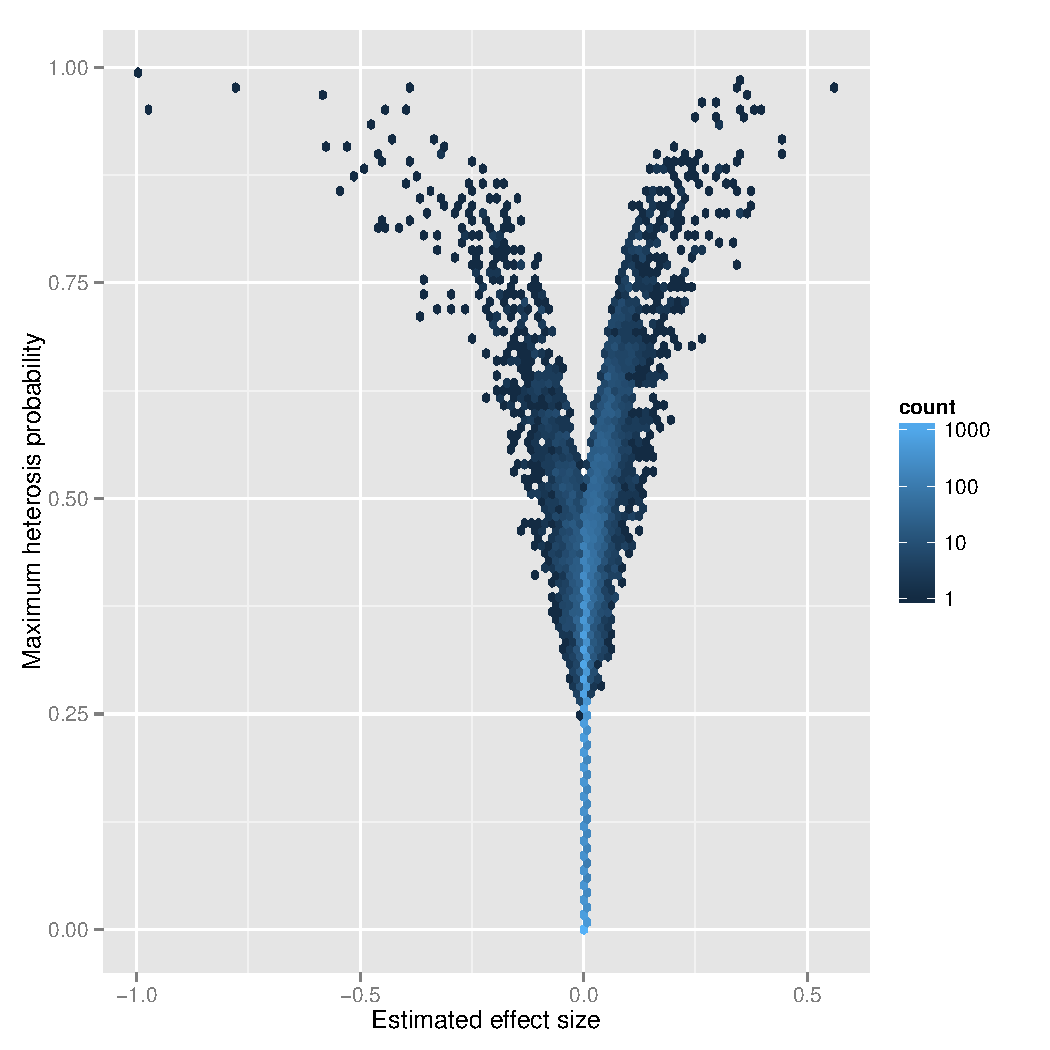
\includegraphics[width=\textwidth]{maize_volcano_dexp}}
\caption{A bivariaet histogram of the maximum of the LPH and HPH probabilities versus estimated effect size defined in equation \ref{e:effect_size} for the B73 $\times$ Mo17 maize experiment.}
\label{f:volcano}
\end{figure}

With almost 30,000 genes in our data set, we can evaluate the distribution assumptions for the gene-specific parameters. Figure \ref{f:scatterplot} provides marginal and bivariate histograms for the gene-specific parameters.


\begin{figure}
\centerline{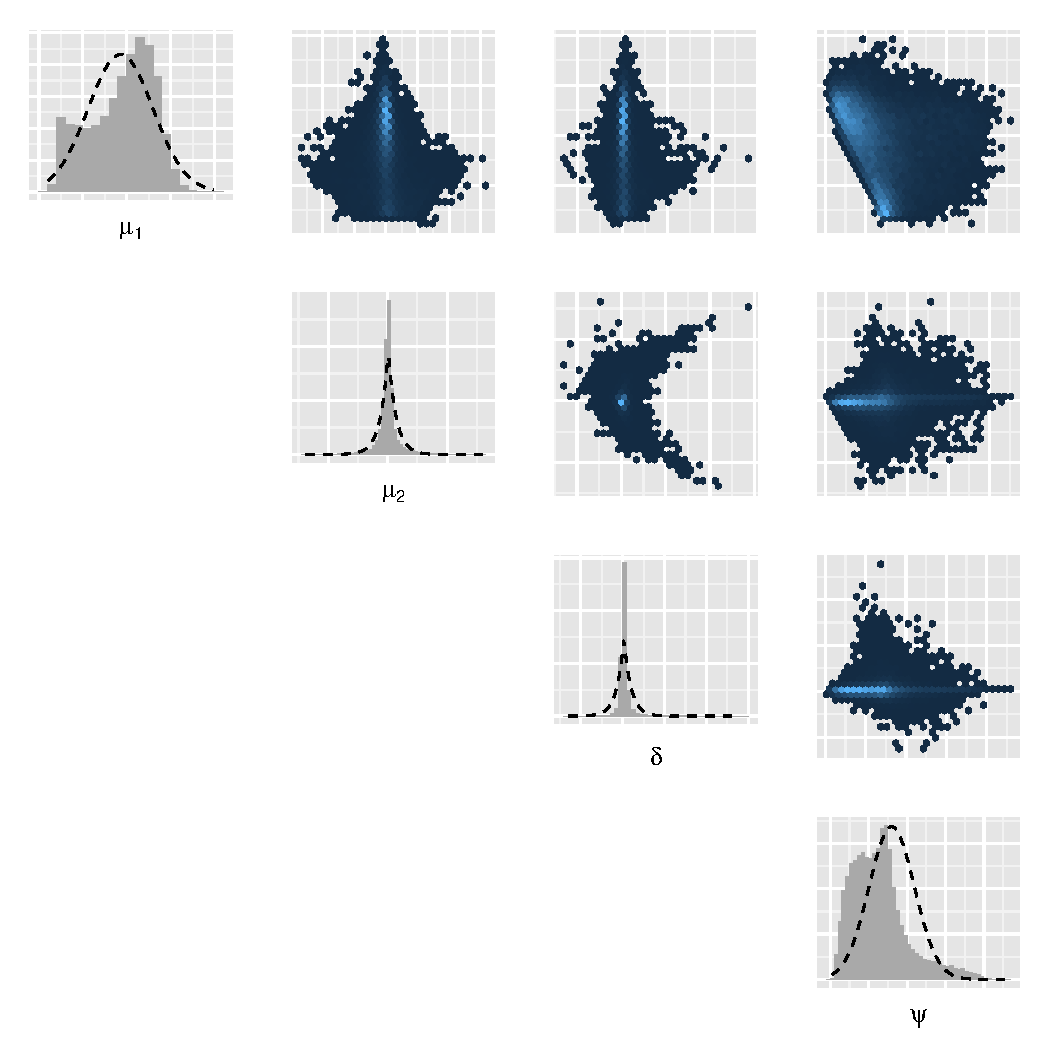
\includegraphics[width=\textwidth]{scatterplot_dexp}}
\caption{Marginal and bivariate histograms for gene-specific parameter posterior meansfor the B73 $\times$ Mo17 maize experiment. For reference, the marginal histograms have a dashed line indicating the appropriate marginal probability density functions in the hierarchical model with the MAP estimates.}
\label{f:scatterplot}
\end{figure}

Marginal and bivariate histograms for the model with an estimated covariance look similar although the estimated distribution $N(\hat{\eta},\hat{\Sigma})$ has increased variance for $\mu$ and decreased variance for $\psi$ as was previously seen in Table \ref{t:map} (results not shown). 

\section{Discussion}
\label{s:discussion}

Geneticists speculate that gene expression heterosis is one possible explanation of phenotypic heterosis of traits, such as plant height or grain yield. Existing methods for identifying differential gene expression based on \RNAseq{} data are not directly applicable for detecting heterosis genes. \cite{ji2014estimation} introduced an empirical Bayes approach based on a hierarchical model for microarray data. We followed their approach, modified to allow for \RNAseq{} read counts as measures of transcript abundance. We developed an empirical Bayes approach based on obtaining MAP estimates for hyperparameters followed by MCMC to estimate gene-specific parameters. This methodology can be conveniently implemented in the statistical software, {\tt Stan}. The empirical Bayes posteriors can be used to estimate posterior probabilities of high and low parent heterosis.  

Through a simulation study, we demonstrated that this method outperformed alternative methods (that are not designed to detect heterosis), and performed comparably well with an implementation of our model in \ShrinkBayes{}, which estimates the full posterior via INLA. We then demonstrated the use of the methodology on a maize experiment in which phenotypic heterosis is well known. 
% Estimates of heterosis to compare with Ji et. al.
In addition to providing estimates of heterosis probabilities and effect sizes, this real data analysis exposed violations of our normality assumptions, indicating room to improve the model and increase the power to detect gene expression heterosis. Some of our ongoing and future research will develop the details of such an extension.





\backmatter %  Please keep this command in your document in this position 

\if0\blind{
\section*{Acknowledgements}

The authors thank Andrew Lithio for help in implementing our model in \ShrinkBayes{}. Research reported in this publication was supported by National Institute of General Medical Sciences of the National Institutes of Health under award number R01GM109458. The content is solely the responsibility of the authors and does not necessarily represent the official views of the National Institutes of Health.
} \fi

%  If your paper refers to supplementary web material, then you MUST
%  include this section!!  See Instructions for Authors at the journal
%  website http://www.biometrics.tibs.org

\section*{Supplementary Materials}

The supplementary materials include the maize experiment data ({\tt data.csv}), a script to run our method ({\tt script.R}), and the {\tt Stan} models: the all-genes-independent (\verb@model_ind.txt@) and covariance (\verb@model_cov.txt@) models used in obtaining MAP estimates, along with the single-gene-independent (\verb@sg_model_ind.txt@) and covariance (\verb@sg_model_cov.txt@) models used in performing the MCMC on single genes. 

\bibliography{jarad}
\bibliographystyle{biom}

% From Dan, "There are some capitalization issues in the references section.  I think you need to protect "RNA" with curly braces so that it stays capitalized.  Also, in Hallauer et al. (2010), the last initial should presumably be "D." rather than "d."."

% \appendix
% %  To get the journal style of heading for an appendix, mimic the following.
% \section{}
% \subsection{Material here}

\label{lastpage}

\end{document}
